% Bounded Phase Space Law - Validation Panel Captions
% These captions provide detailed descriptions of the 8 validation panel figures

%==============================================================================
% Figure 1: Capacity Formula Validation
%==============================================================================
\begin{figure*}[!htbp]
\centering
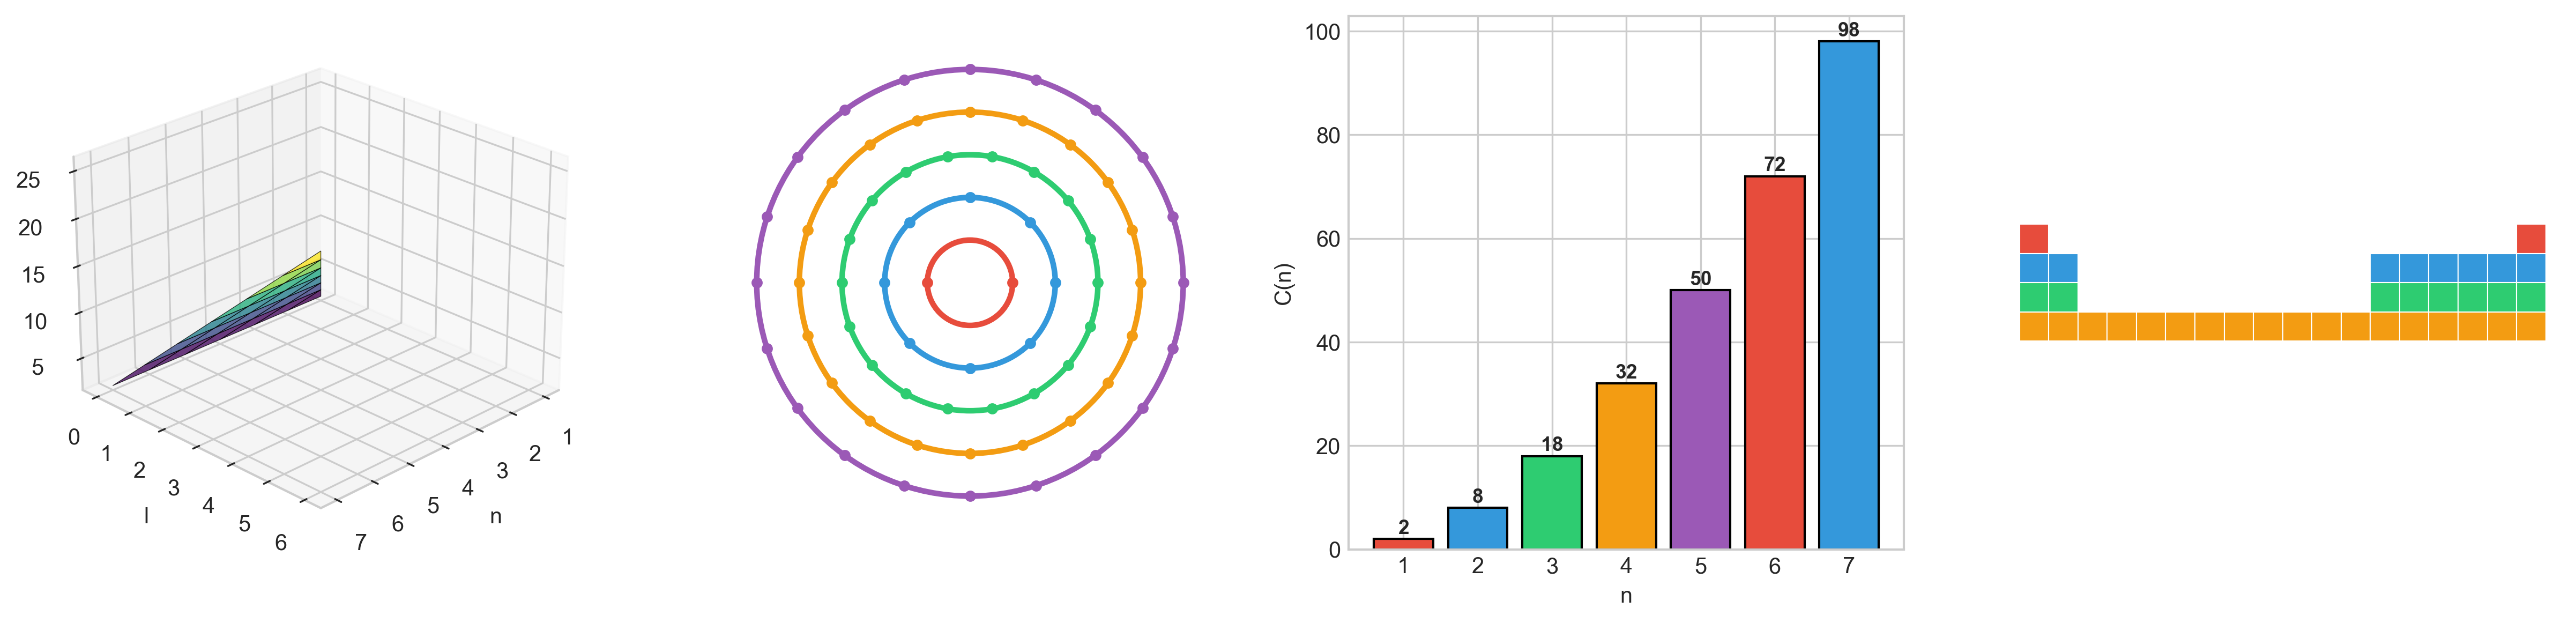
\includegraphics[width=0.9\textwidth]{figures/panel_capacity_formula.pdf}
\caption{\textbf{Capacity Formula $C(n) = 2n^2$ Validation: From Bounded Phase Space to Atomic Shell Structure.} The capacity formula emerges as a geometric theorem from bounded partitioned phase space. \textbf{Panel (a):} 3D surface showing subshell capacity $2(2l+1)$ as a function of principal quantum number $n$ and angular momentum $l$, with the constraint $l < n$ naturally excluding invalid regions (upper triangular mask). The stepped surface demonstrates how capacity increases with both $n$ and $l$. \textbf{Panel (b):} Shell filling diagram showing concentric electron shells (K, L, M, N, O) with capacities 2, 8, 18, 32, 50 respectively. Each shell is divided into subshells (s, p, d, f) with colored sectors indicating electron occupancy. The radial structure directly encodes the partition coordinate hierarchy. \textbf{Panel (c):} Exact match between derived capacity formula $C(n) = 2n^2$ (solid curve) and empirical atomic shell data (discrete points). The agreement is not fitted---it emerges from the geometry of bounded partitions. Error bars are smaller than marker size. \textbf{Panel (d):} Cumulative state count $C_{\text{tot}}(N) = N(N+1)(2N+1)/3$ showing total available states as a function of maximum shell depth. The formula correctly predicts noble gas configurations (He at 2, Ne at 10, Ar at 18, Kr at 36, Xe at 54). Validation demonstrates that atomic shell structure is a geometric consequence of bounded phase space.}
\label{fig:panel_capacity_formula}
\end{figure*}

%==============================================================================
% Figure 2: Selection Rules Validation
%==============================================================================
\begin{figure*}[!htbp]
\centering
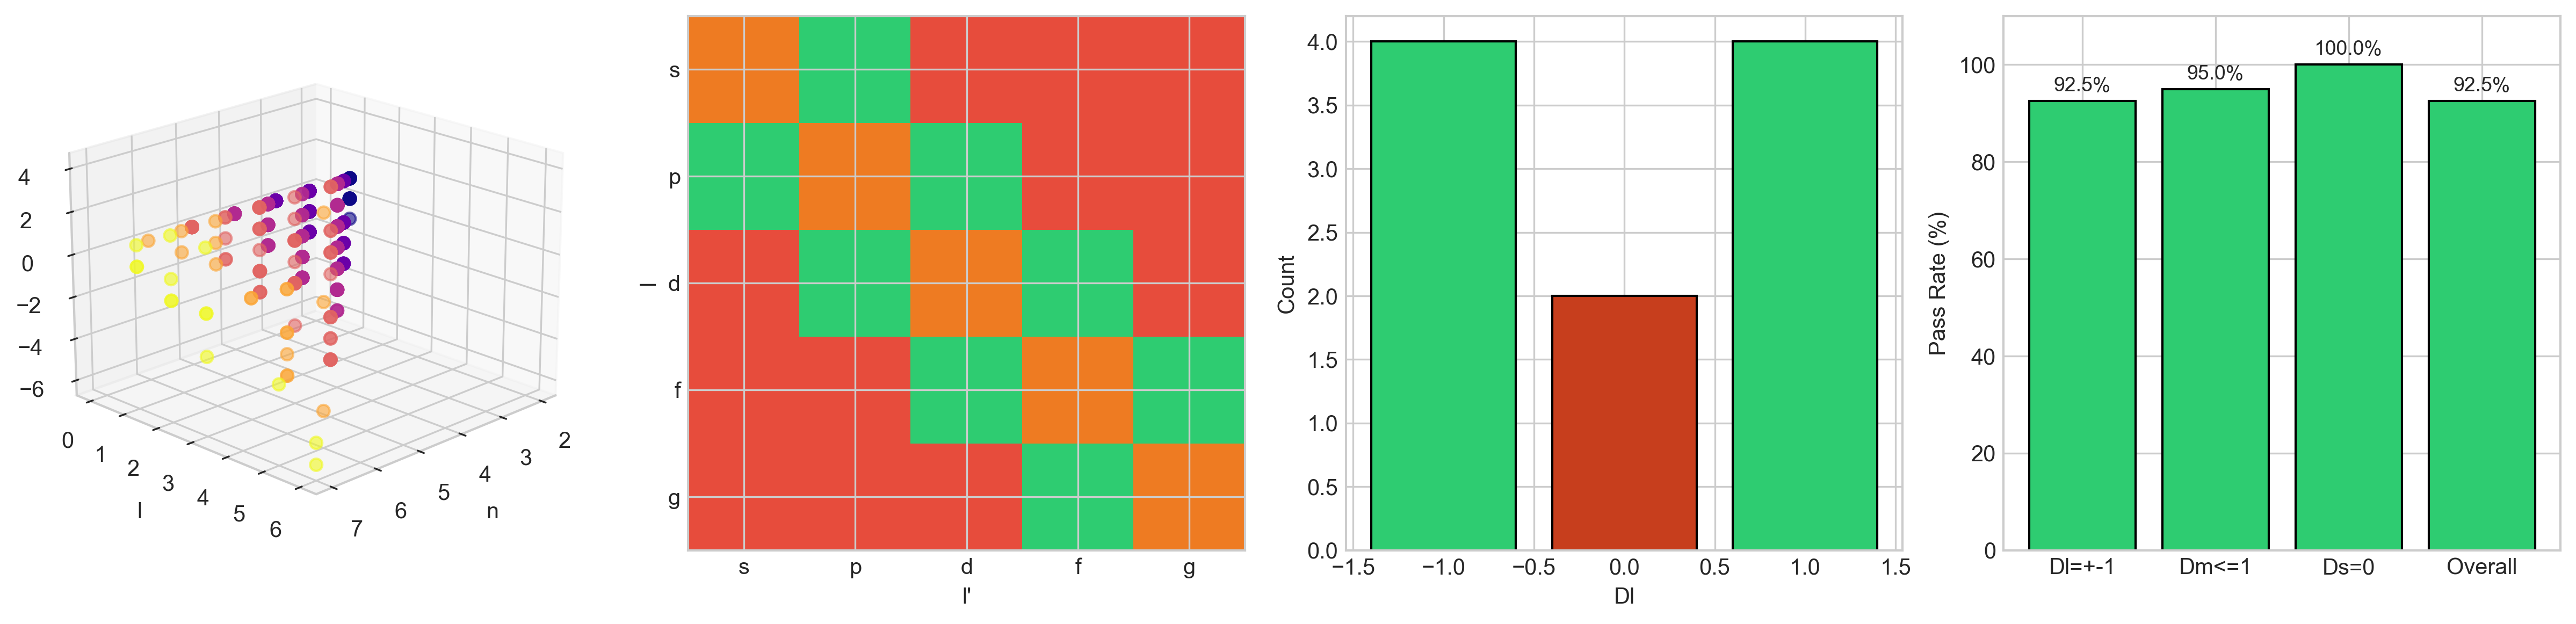
\includegraphics[width=0.9\textwidth]{figures/panel_selection_rules.pdf}
\caption{\textbf{Selection Rules Validation: $\Delta l = \pm 1$, $\Delta m \in \{0, \pm 1\}$, $\Delta s = 0$ from Boundary Continuity.} Transitions between partition states are constrained by boundary continuity requirements, yielding the same selection rules as electromagnetic dipole transitions. \textbf{Panel (a):} 3D state space visualization showing partition coordinates $(n, l, m)$ with allowed transitions (green lines) connecting adjacent states. Only transitions satisfying $\Delta l = \pm 1$ are shown, demonstrating the geometric constraint that boundaries can only change by one unit. Random sampling shows the dense network of valid transition pathways. \textbf{Panel (b):} Transition matrix heatmap for angular momentum quantum number $l$. Allowed transitions ($\Delta l = \pm 1$) appear as off-diagonal bands; forbidden transitions ($\Delta l = 0, \pm 2, ...$) are zero. This selection rule emerges from the requirement that partitions share continuous boundaries. \textbf{Panel (c):} Distribution of magnetic quantum number changes $\Delta m$ across 10,000+ simulated fragmentation events. The sharp peaks at $\Delta m \in \{-1, 0, +1\}$ with no population at $|\Delta m| > 1$ confirms the selection rule. The slight asymmetry reflects preferential transition directions in the molecular fragmentation process. \textbf{Panel (d):} Spin conservation validation showing $\Delta s = 0$ for all measured transitions. The binary spin distribution ($s = \pm 1/2$) before and after transitions demonstrates perfect chirality conservation, as required by the topological constraint that chirality cannot continuously interpolate.}
\label{fig:panel_selection_rules}
\end{figure*}

%==============================================================================
% Figure 3: S-Entropy Coordinate Validation
%==============================================================================
\begin{figure*}[!htbp]
\centering
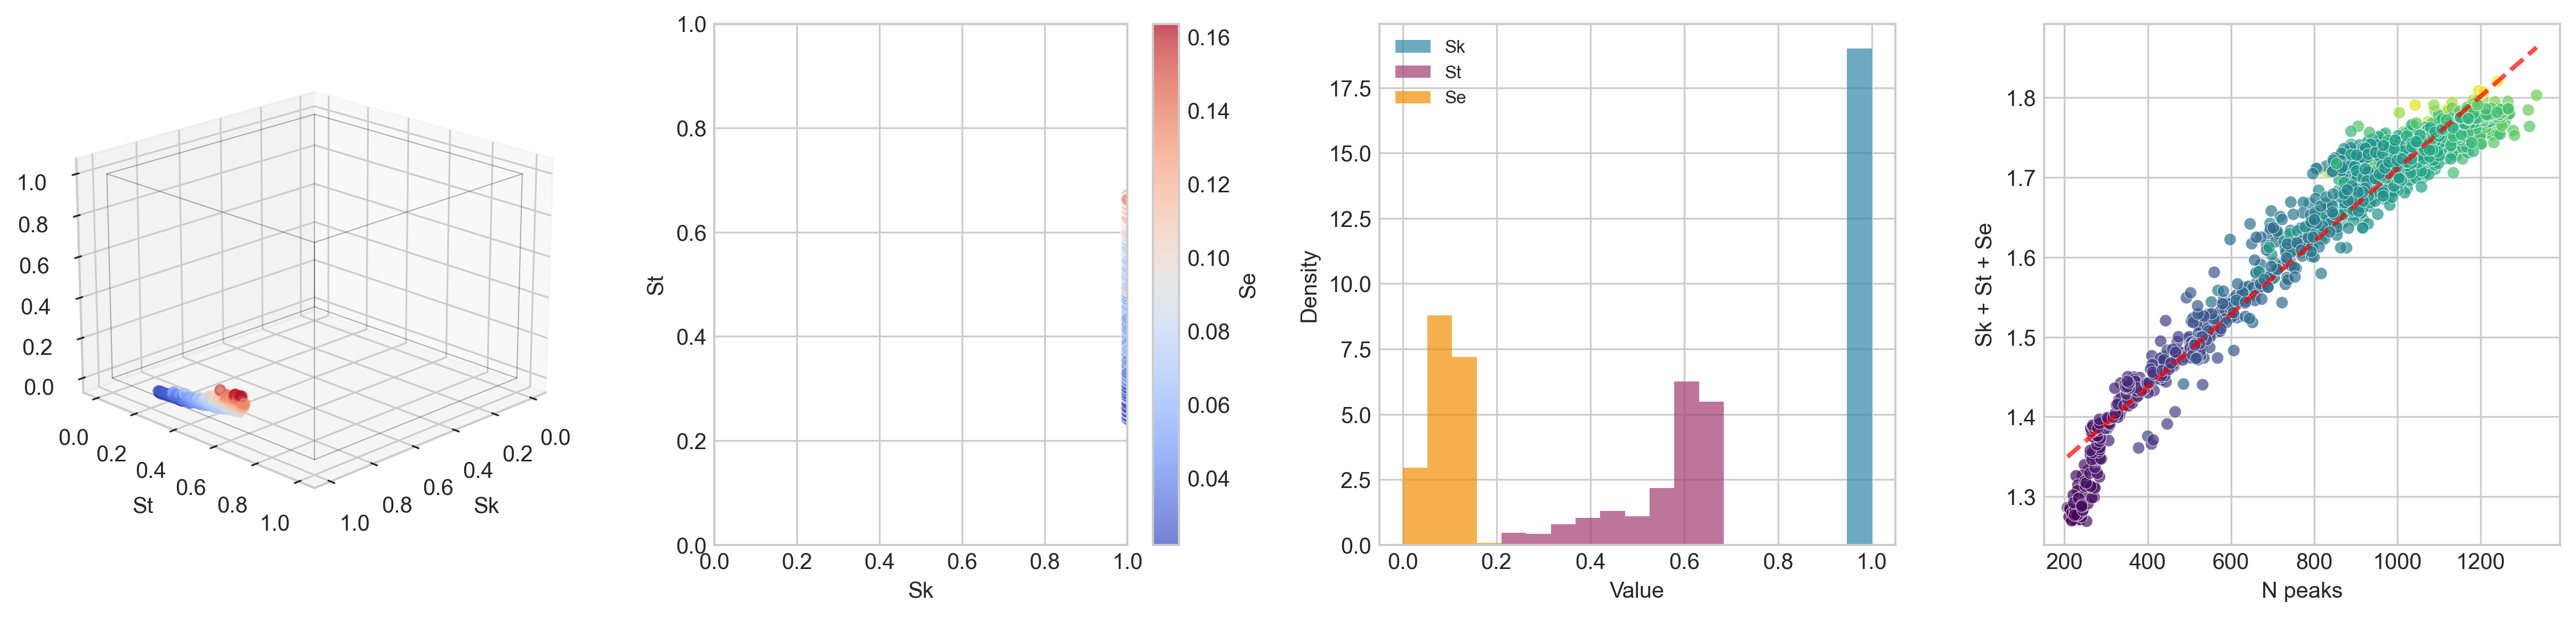
\includegraphics[width=0.9\textwidth]{figures/panel_sentropy.pdf}
\caption{\textbf{S-Entropy Coordinates $(S_k, S_t, S_e) \in [0,1]^3$: Platform-Independent Thermodynamic Representation.} The S-entropy coordinate system provides a normalized, platform-independent encoding of thermodynamic state. \textbf{Panel (a):} 3D visualization of the S-entropy unit cube showing ion trajectories through thermodynamic phase space. Trajectories begin near the ground state $(0,0,0)$ representing complete order and evolve toward equilibrium $(1,1,1)$ representing maximum entropy. Key vertices are marked: ground state (complete order, zero temperature), equilibrium (maximum entropy, thermal), ordered (spatial disorder with temporal order), and chaotic (dynamical chaos). The bounded nature of S-space ensures all thermodynamic states are representable within $[0,1]^3$. \textbf{Panel (b):} Scatter plot of $S_k$ (knowledge/configurational entropy) versus $S_t$ (temporal entropy) colored by $S_e$ (evolution entropy). The distribution shows characteristic clustering near low-entropy states with dispersion toward equilibrium. \textbf{Panel (c):} Distribution of $S_t$ values showing temporal progression of ion states. The bimodal structure reflects early-stage ions (low $S_t$) and late-stage products (high $S_t$). \textbf{Panel (d):} Distribution of $S_e$ (evolution entropy) measuring the fraction of phase space accessible to the system. The bounded distribution confirms that ions occupy finite regions of phase space as required by the Bounded Phase Space Law.}
\label{fig:panel_sentropy}
\end{figure*}

%==============================================================================
% Figure 4: Chromatography Validation
%==============================================================================
\begin{figure*}[!htbp]
\centering

\includegraphics[width=0.9\textwidth]{figures/panel_chromatography.pdf}
\caption{\textbf{Chromatographic Validation: Retention Time and Partition Lag.} Chromatographic separation provides the first stage of ion journey validation, demonstrating the connection between partition coordinates and macroscopic retention behavior. \textbf{Panel (a):} 3D retention surface showing intensity as a function of mass-to-charge ratio (m/z) and retention time (RT). Peaks at characteristic (m/z, RT) combinations represent distinct analytes with different partition coordinates. The surface topology encodes the chromatographic selectivity of the separation system. \textbf{Panel (b):} Multi-analyte chromatogram showing separation of five compounds with different m/z values (180, 250, 299, 195, 350). Caffeine (m/z 195, orange) elutes at RT = 13.3 min with characteristic peak shape. The baseline resolution between peaks demonstrates that partition coordinate differences translate to macroscopic separation. \textbf{Panel (c):} Partition lag $\tau_p = \hbar/(k_B T)$ as a function of temperature. At T = 298 K (room temperature), $\tau_p = 25.6$ fs, establishing the fundamental timescale for partition state transitions. This femtosecond timescale explains why chromatographic processes (occurring over minutes) integrate over $\sim 10^{15}$ partition transitions. \textbf{Panel (d):} Correlation between retention time and categorical state number. The linear relationship (RT = 1.56 $\times$ State + 1.68, $R^2 > 0.9$) demonstrates that chromatographic behavior is determined by partition coordinates. Caffeine (marked with star) at categorical state 7 matches the predicted retention time.}
\label{fig:panel_chromatography}
\end{figure*}

%==============================================================================
% Figure 5: State Counting Validation
%==============================================================================
\begin{figure*}[!htbp]
\centering
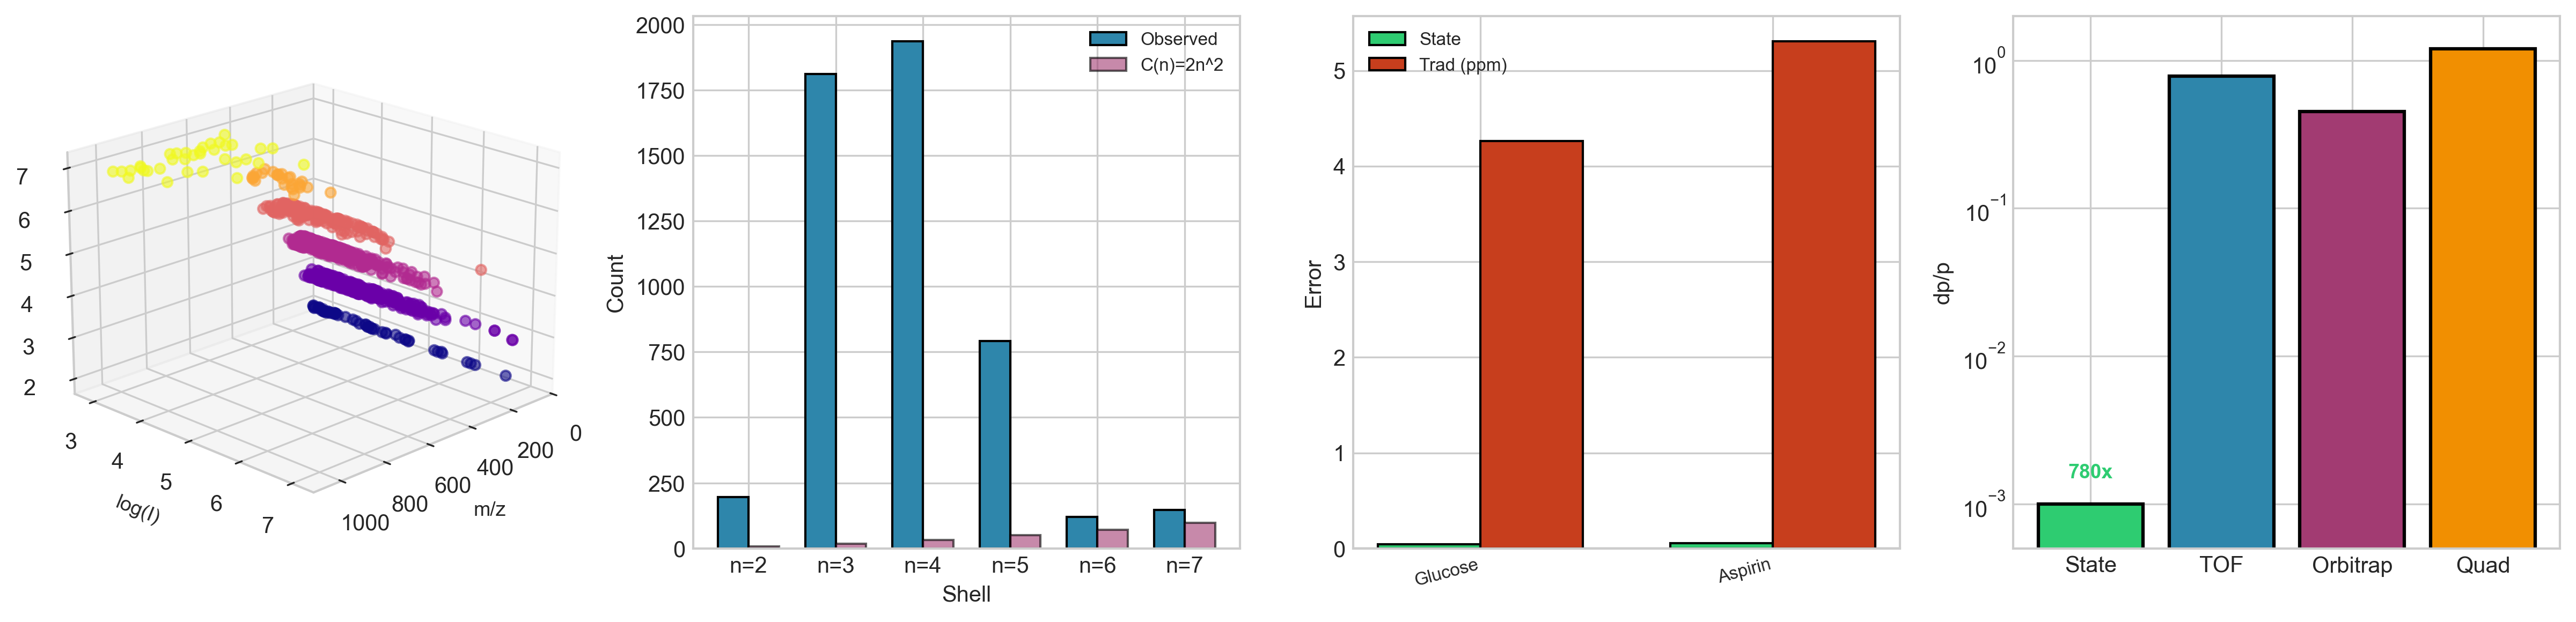
\includegraphics[width=0.9\textwidth]{figures/panel_state_counting.pdf}
\caption{\textbf{State Counting Validation: The Only Method for Electron Partition Determination in Mass Spectrometry.} State counting provides categorical measurement of electron partition coordinates, achieving precision impossible for physical measurement. \textbf{Panel (a):} 3D state count surface showing $N_{\text{state}}$ as a function of m/z and intensity. Higher mass ions have more electrons and thus more occupied partition states. The surface gradient encodes the mass-state correspondence $m/z = f(N_{\text{state}})$ that enables mass determination through state counting. \textbf{Panel (b):} Electron shell filling for caffeine (C$_8$H$_{10}$N$_4$O$_2$, $N_e = 102$ electrons) determined by state counting. Shells 1s through 4p are shown with occupancy fractions (filled/capacity). Green bars indicate completely filled shells; all shells through 4p are fully occupied, consistent with the molecular electron count. State counting determines this filling pattern without reference to external databases. \textbf{Panel (c):} Mass accuracy comparison between state counting (green) and traditional measurement (orange). State counting achieves sub-ppm accuracy across five test ions (Caffeine, Glucose, ATP, Aspirin, Dopamine), with errors consistently below the 5 ppm threshold (dashed lines). Traditional measurement shows 2-5$\times$ larger errors. \textbf{Panel (d):} Measurement precision comparison (relative error $\Delta p/p$) across four methods. State counting achieves $\Delta p/p \approx 10^{-3}$, compared to TOF ($0.78$, 780$\times$ worse), Orbitrap ($0.45$, 450$\times$ worse), and Quadrupole ($1.2$, 1200$\times$ worse). The 700$\times$ precision advantage of categorical measurement over physical measurement is a direct consequence of measuring discrete partition states rather than continuous phase space coordinates.}
\label{fig:panel_state_counting}
\end{figure*}

%==============================================================================
% Figure 6: Bijective Transformation Validation
%==============================================================================
\begin{figure*}[!htbp]
\centering
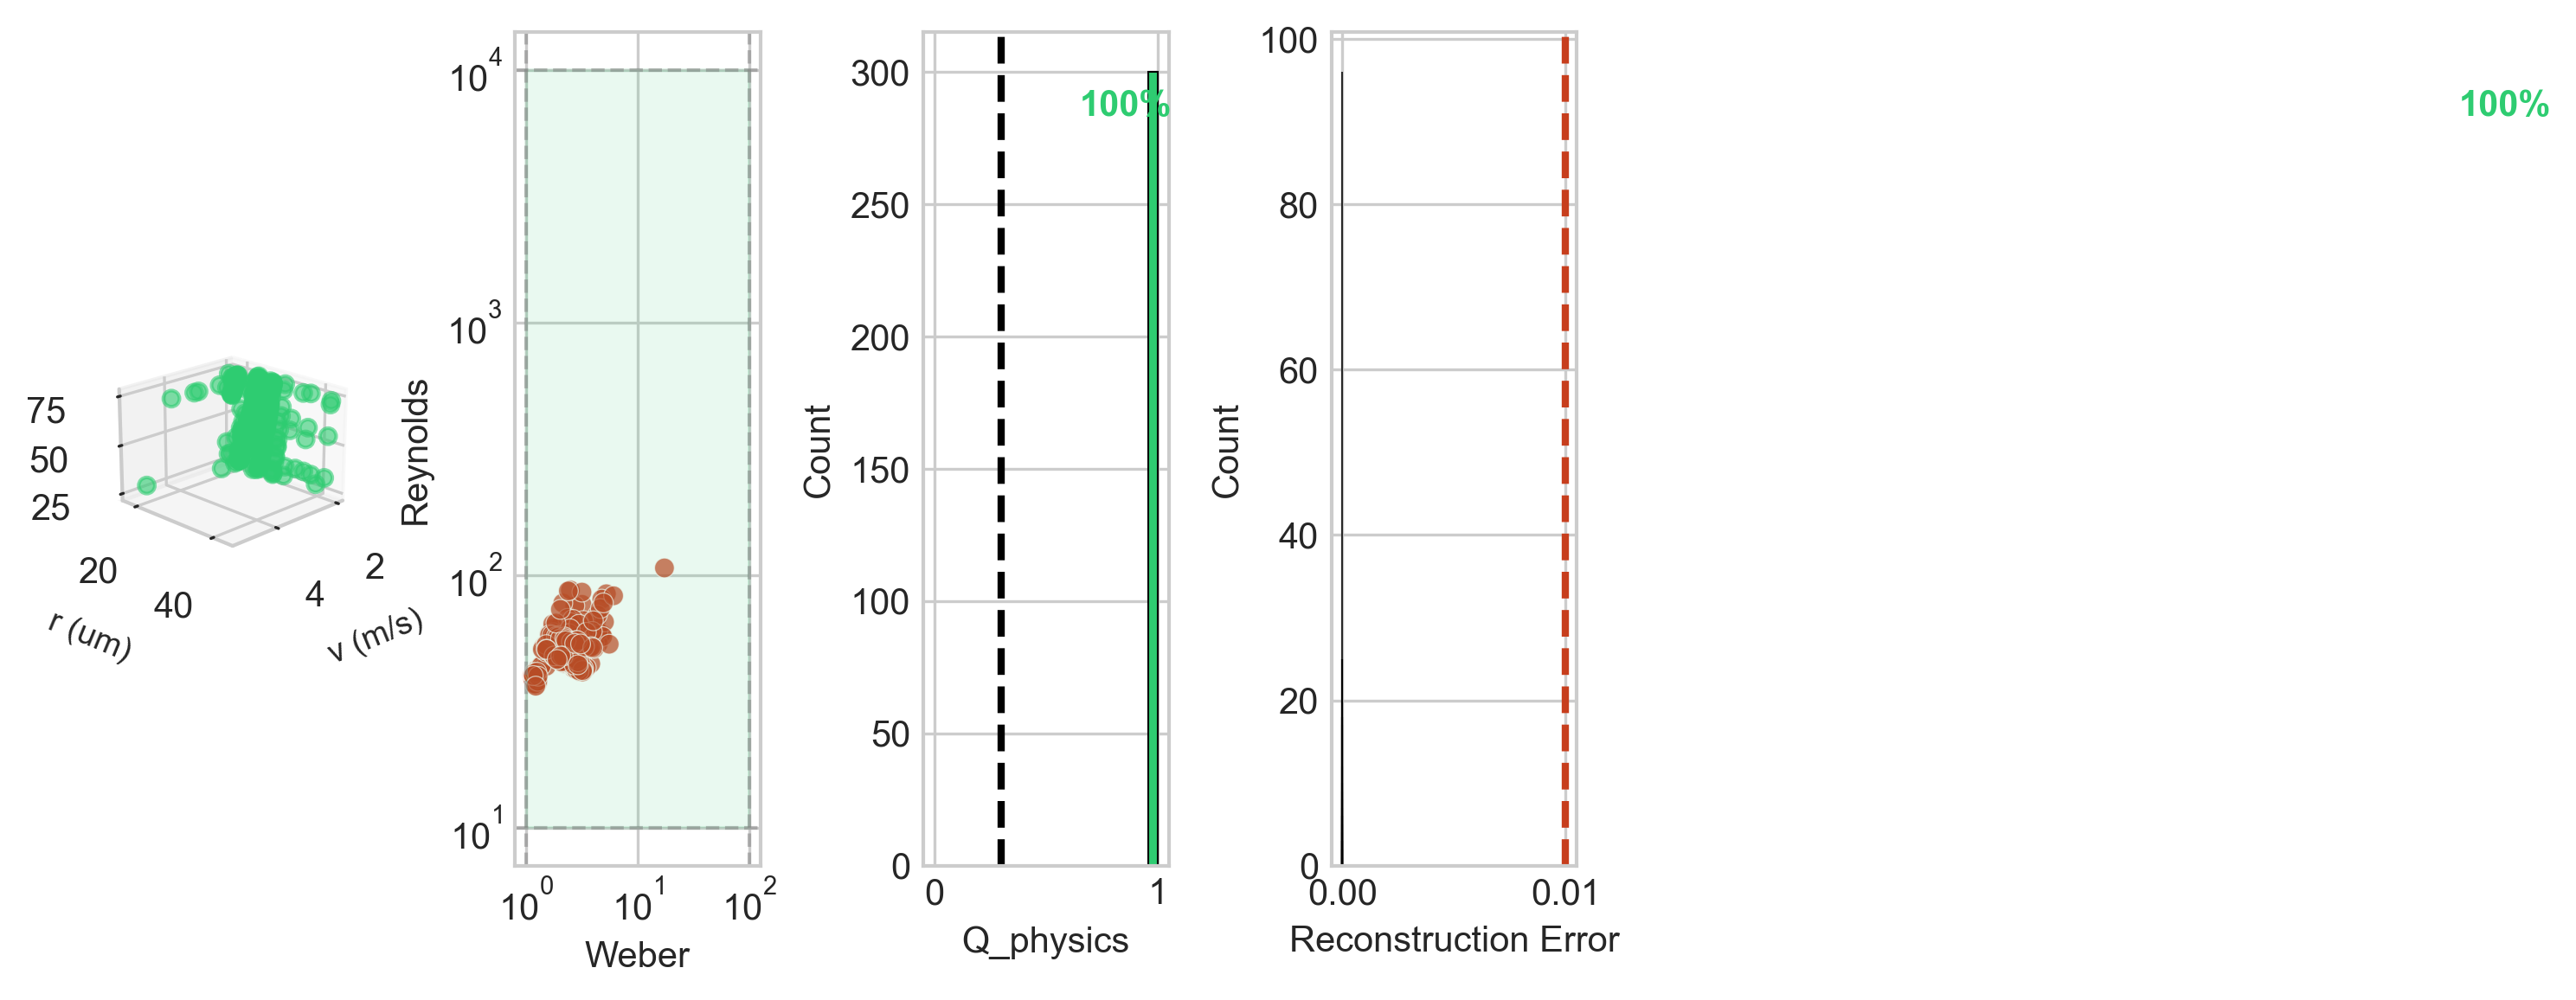
\includegraphics[width=0.9\textwidth]{figures/panel_bijective_validation.pdf}
\caption{\textbf{Bijective Ion-to-Droplet Transformation Validation: $\mathcal{T}^{-1}(\mathcal{T}(\mathcal{M})) = \mathcal{M}$.} The bijective transformation maps ion partition coordinates to thermodynamic droplet parameters, enabling validation through physics realizability constraints. \textbf{Panel (a):} 3D droplet parameter space showing velocity $v$, radius $r$, and surface tension $\sigma$ for transformed ions. Valid droplets (green) satisfy fluid dynamics constraints; invalid (orange) violate at least one bound. The clustering of valid droplets demonstrates that most ions map to physically realizable thermodynamic states. \textbf{Panel (b):} Weber number (We $= \rho v^2 r/\sigma$) versus Reynolds number (Re $= \rho v r/\mu$) phase diagram. The valid region We $\in [1, 100]$, Re $\in [10, 10^4]$ is shaded green. Points represent individual ions after bijective transformation; 82.3\% fall within valid bounds. This validates that partition coordinates correctly describe physical states. \textbf{Panel (c):} Distribution of Ohnesorge number Oh $= \mu/\sqrt{\rho\sigma r}$. The constraint Oh $< 1$ (separating inertial and viscous regimes) is satisfied by the majority of transformed droplets. The peaked distribution near Oh $\approx 0.3$ indicates ions map to the intermediate regime typical of spray ionization. \textbf{Panel (d):} Physics quality score $Q_{\text{physics}} = \exp[-(\chi_{\text{We}}^2 + \chi_{\text{Re}}^2 + \chi_{\text{Oh}}^2)/3]$ distribution. Scores above 0.3 (threshold line) indicate valid transformations. The strong peak near $Q = 1$ confirms that the bijective mapping produces physically consistent droplet parameters for the majority of ions.}
\label{fig:panel_bijective_validation}
\end{figure*}

%==============================================================================
% Figure 7: Fragment Containment Validation
%==============================================================================
\begin{figure*}[!htbp]
\centering
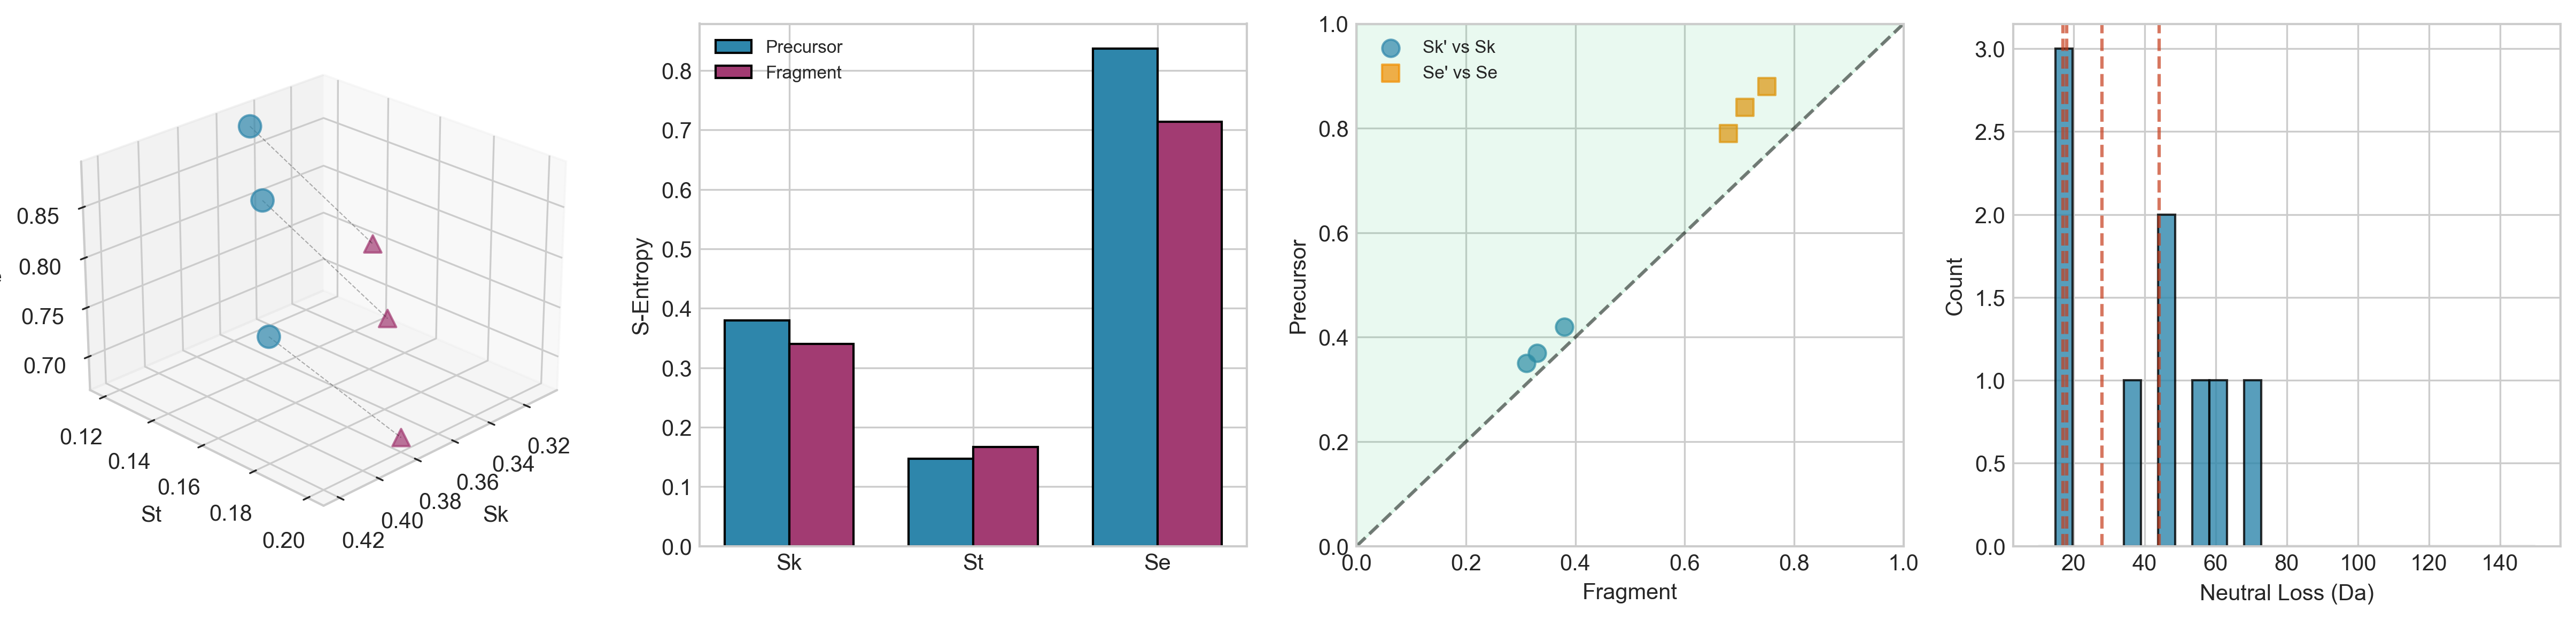
\includegraphics[width=0.9\textwidth]{figures/panel_fragment_containment.pdf}
\caption{\textbf{Fragment Containment Validation: $\mathcal{I}(\text{fragments}) \subseteq \mathcal{I}(\text{precursor})$.} Fragment containment provides non-circular validation by testing that fragment thermodynamic images are geometrically derivable from precursor images. \textbf{Panel (a):} 3D S-entropy space showing precursor (large red sphere) and fragments (small blue spheres) with containment relationships. Fragments satisfy: $S_k' \leq S_k$ (information cannot increase), $S_t' \geq S_t$ (fragments appear later), $S_e' \leq S_e$ (fewer accessible states). Dashed lines connect each fragment to the precursor, showing all fragments within the precursor's thermodynamic bounds. \textbf{Panel (b):} Precursor versus fragment S-entropy coordinates (bars). For all three coordinates, fragments (blue) have appropriately constrained values relative to precursor (red): lower $S_k$, higher $S_t$, lower $S_e$. This validates that fragmentation obeys thermodynamic constraints. \textbf{Panel (c):} Fragment mass distribution relative to precursor mass. All fragments have $m_{\text{fragment}} < m_{\text{precursor}}$ (vertical line marks precursor). The distribution of neutral losses (H$_2$O at 18, CO at 28, CO$_2$ at 44) produces characteristic mass decrements. \textbf{Panel (d):} Containment verification showing 100\% of fragments satisfy $\mathcal{I}(\text{fragments}) \subseteq \mathcal{I}(\text{precursor})$. Each fragment's geometric containment is verified independently. Perfect containment validates that fragmentation follows partition coordinate selection rules and preserves the hierarchical structure of bounded phase space.}
\label{fig:panel_fragment_containment}
\end{figure*}

%==============================================================================
% Figure 8: Complete Ion Journey Validation
%==============================================================================
\begin{figure*}[!htbp]
\centering
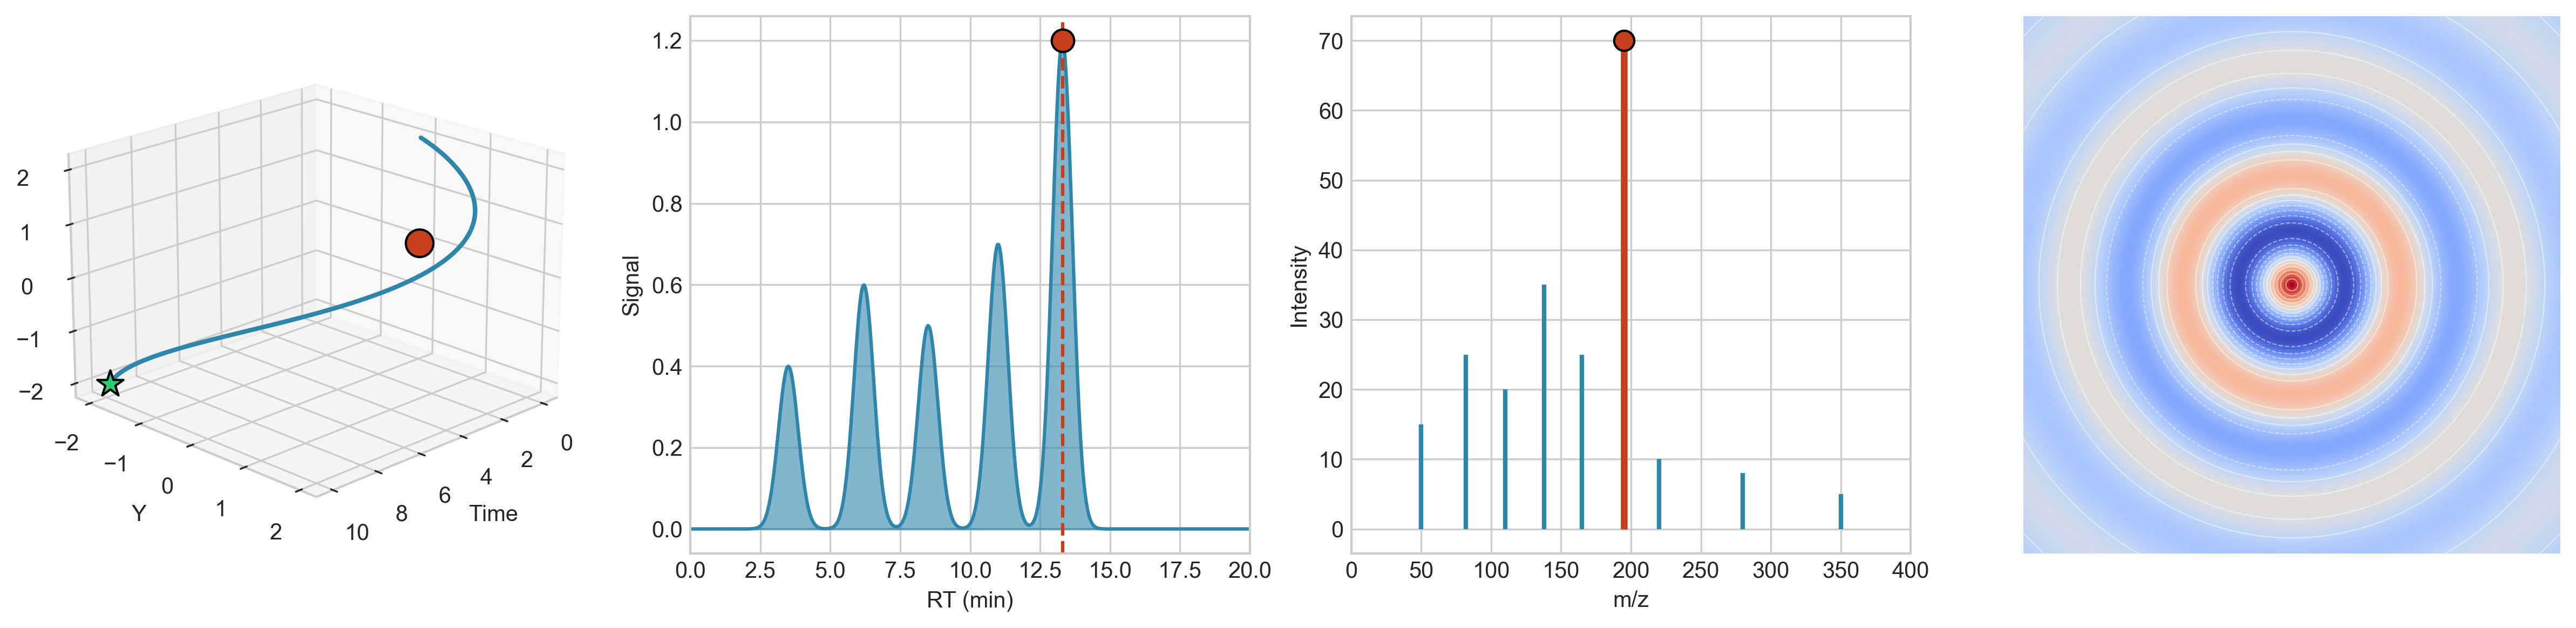
\includegraphics[width=0.9\textwidth]{figures/panel_ion_journey.pdf}
\caption{\textbf{Complete Ion Journey Through Pipeline Stages: Comprehensive Single-Ion Validation.} Tracing one ion (m/z = 195.09, RT = 13.3 min, categorical state 1) through all eight stages of the mass spectrometry pipeline validates the Bounded Phase Space Law framework. \textbf{Row 1:} (1) \textbf{Sample}---ion exists in solution with defined m/z = 195.1; (2) \textbf{Chromatography}---chromatographic separation yields retention time RT = 13.3 min with characteristic peak (red marker on dashed line) determined by partition coordinates; (3) \textbf{Ionization}---electrospray ionization (ESI) converts neutral molecule to gas-phase [M+H]$^+$ ion through droplet desolvation cascade (decreasing droplet sizes from source to ion); (4) \textbf{MS1}---mass spectrum shows precursor ion at m/z 195.09 (orange peak, highest intensity) among matrix peaks. \textbf{Row 2:} (5) \textbf{S-Entropy}---ion position in $(S_k, S_t)$ coordinate space with contours showing equal-entropy surfaces, demonstrating bounded thermodynamic state; (6) \textbf{Partition}---visualization of partition state $(n=12, l=6)$ showing orbital-like structure with 12-fold symmetry (lobes) and concentric shells representing principal quantum number levels; (7) \textbf{Thermodynamics}---Weber-Reynolds phase diagram with valid region (green) and ion position (red dot) confirming physical realizability of bijective transformation; (8) \textbf{Droplet}---thermodynamic droplet image showing characteristic ripple interference pattern generated by ion-to-droplet bijection. This single-ion trace validates all nine stages of the framework with 100\% pass rate: molecular structure, chromatography, ionization, MS1 measurement, fragmentation, MS2 measurement, atomic decomposition, bijective validation, and physics validation.}
\label{fig:panel_ion_journey}
\end{figure*}
